\section{Engenharia de Software Orientada a Agentes}

A Engenharia de Software Orientada a Agentes (AOSE), está preocupada com a forma de engenharia efetiva de sistemas de agentes, isto é, como especificar, projetar, implementar, verificar e manter estes softwares \citep{winikoff2009future}. \citet{sturm2014agent} apresenta as áreas de atuação da AOSE representada pela Figura \ref{fig:aose_areas}.

\begin{figure}[ht]
\centering
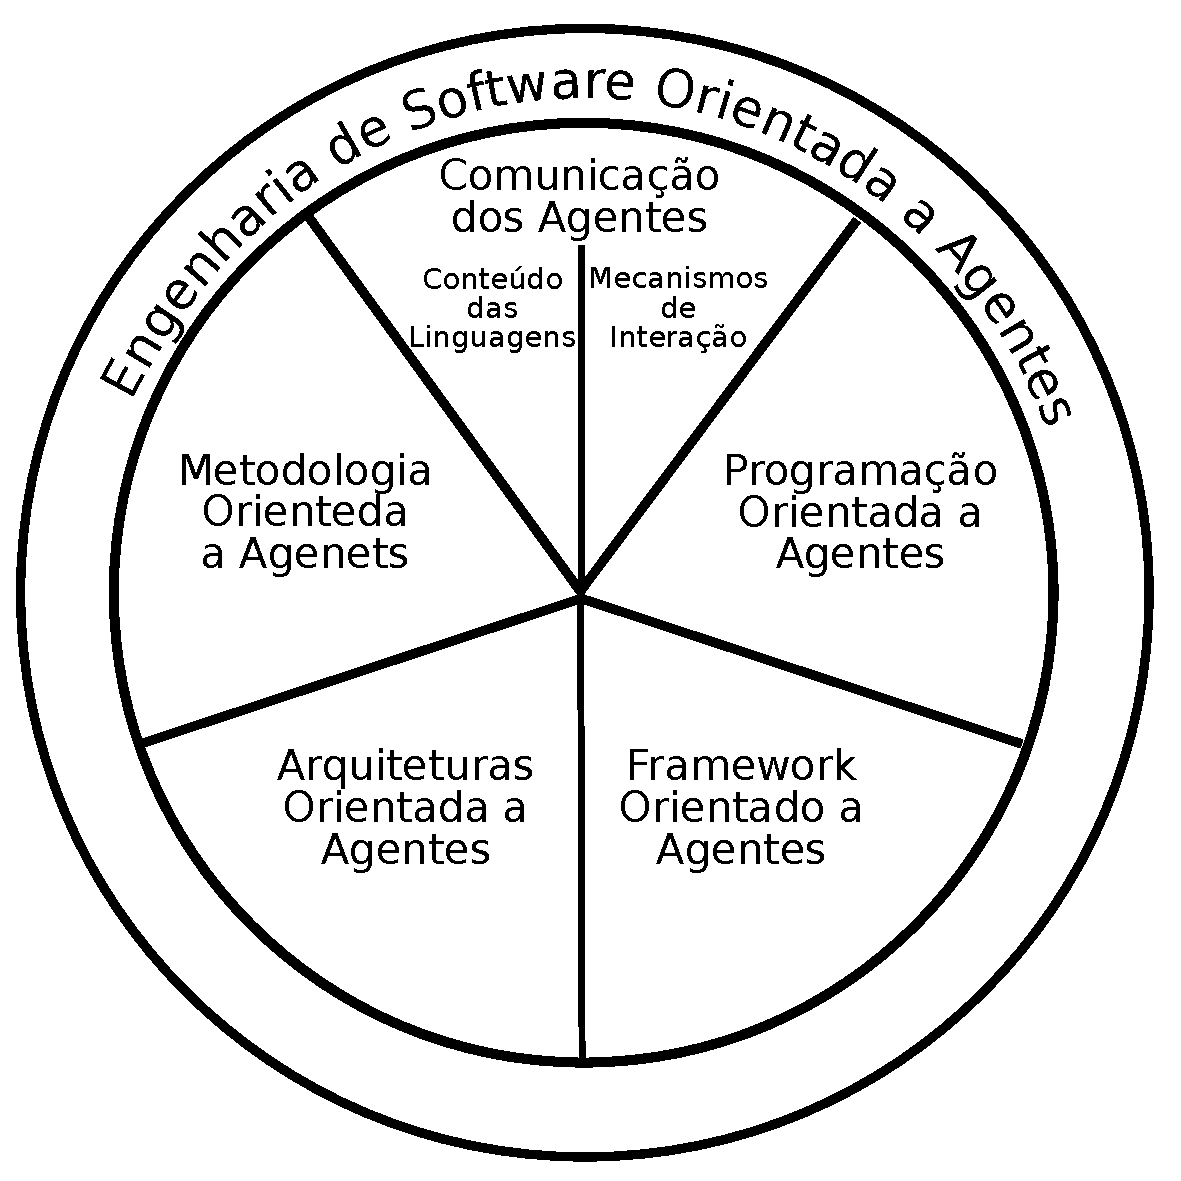
\includegraphics[scale=0.45]{imagens/aose.pdf}
\caption{Atuação da AOSE}
\label{fig:aose_areas}
\end{figure}

\subsection{Metodologias AOSE}

Segundo \citep{padgham2016agent} muitos autores veêm os agentes de software como uma evolução dos objetos promovendo uma abstração e encapsulamento, e deste modo ocorreram tentativas de desenvolver metodologias para o desenvolvimento de software baseado em agentes aproveitando técnicas da engenharia de software tradicional. 

Para \citet{akbari2010survey} uma metodologia de engenharia de software orientada por agente é um processo comercial de desenvolvimento de software, equipado com conceitos distintos e ferramentas de modelagem, nas quais a chave é a abstração usada em seus conceitos que é a de um agente. Apesar de AOSE já existir pelo menos há duas décadas muito ainda tem a ser feito para uma adoção maior da indústria. Alguns pontos a serem melhorados \cite{sturm2014agent}:

\begin{itemize}
\item Definição de um conjunto central de propriedades dos agentes.
\item Esclarecer como a AOSE pode facilitar o gerenciamento da complexidade na Engenharia de Software.
\item Padronização das técnicas de AOSE já desenvolvidas
\item Maior integração de tecnologia multi-agentes com as tecnologias já utilizadas na indústria.
\end{itemize}

Além desses pontos que exigem uma grande atenção para uma maior adoção do mercado, \citet{sturm2014landscape} reforça que as metodologias orientadas a agentes atuais focam seus esforços no desenvolvimento de novos sistemas e não nos outros estágios e aspectos de ciclo de vida do sistema, como são compreendidos na engenharia de software tradicional. O teste de software e o aspecto de manutenção do sistema dificilmente são suportado dentro das metodologias orientada a agentes.

\begin{table}[h]
\centering
\caption{Metodologias AOSE}
\label{tab:metodologias}
\begin{tabular}{@{}lll@{}}
\toprule
Nome da Metodologia & Ano de Origem & Domínio de Origem \\ \midrule
ADELFE              & 2002          & ES                \\ 
GAIA                & 2000          & ES                \\ 
INGENIAS            & 2002          & ES                \\ 
MaSE                & 1999          & ES                \\ 
MESSAGE             & 2000          & ES                \\ 
Prometheus          & 2002          & ES + IA-EC        \\ 
Tropos              & 2001          & ES+ IA-EC         \\ \bottomrule
\end{tabular}
\end{table}

% * <eder.m.goncalves@gmail.com> 2017-10-20T16:12:04.844Z:
% 
% Definir as siglas da tabela.
% 
% ^.

\subsubsection{Prometheus}

A metodologia Prometheus visa abranger todas as principais atividades nos sistemas de desenvolvimento de agentes, sendo bastante detalhada e completa. Segundo FULANO, esta metodologia tem por objetivo a fácil utilização podendo ser utilizada tanto por usuários especialistas como por usuários não especializados. A metodologia consiste em três fases: especificação do sistema, projeto arquitetônico e projeto detalhado. A Figura \ref{fig:f_prometheus}.
% * <eder.m.goncalves@gmail.com> 2017-10-20T16:13:02.362Z:
% 
% > FULANO
% ?
% 
% ^.

\begin{figure}[ht]
\centering
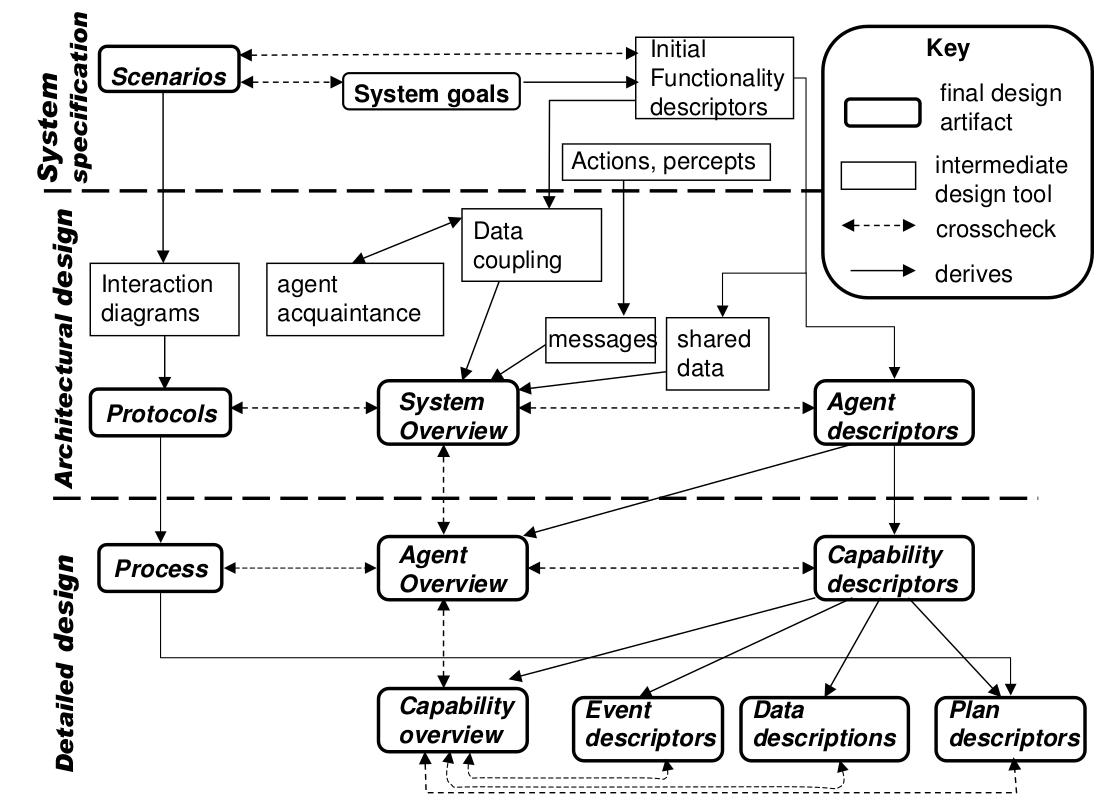
\includegraphics[scale=0.3]{imagens/fases_prometheus.png}
\caption{Fases da metodologia Prometheus }
\label{fig:f_prometheus}
\end{figure}

\begin{itemize}
\item Especificação do Sistema \\
A especificação do sistema é a primeira fase do Prometheus. O objetivo principal é a construção do modelo de ambiente do sistema que é onde o agente está atuando, identificação das metas e as funcionalidades do sistema e descrevendo os principais cenários de casos de uso.

A modelagem de um ambiente envolve duas atividades: identificar percepções que são informações recebidas do meio ambiente e determinar ações que são os meios pelos quais um agente afeta seu ambiente. Percepções e ações são definidas usando descritores. Além disso, recursos externos, tais como dados, informações precisam ser identificados.

Nesta fase as metas e as funcionalidades do sistema precisam ser capturadas. No primeiro passo, as metas do sistema são identificadas principalmente com base na especificação dos requisitos. As metas podem ser decompostas em submetas, se necessário. Depois disso, as funcionalidades do sistema que atingem essas metas são definidas. Outro passo que ajuda os analistas a identificar as funcionalidades do sistema está é por meio de cenários de casos de uso. Estes cenários descrevem exemplos do sistema em operação.

\item Projeto Arquitetônico \\

Nesta fase são definidos os grupos de agentes que existem no sistemas, segundo as suas funcionalidades. As funcionalidades do sistema são agrupadas entre as que se relacionam por critério de coesão ou acoplamento. Depois de definido os grupos de agentes, a estrutura do ambiente é capturada em um diagrama de visão geral do sistema. Este diagrama mostra os tipos de agentes, as comunicações entre eles e os dados usados, apresentando uma visão geral e estática de como o sistema funcionará. Nesta etapa também são gerados diagramas que representam a dinâmica do sistema, o diagrama de interação, baseado nos cenários de casos de uso e protocolos de interação que definem a sequência de mensagem dos agentes.

\item Projeto Detalhado \\

Nesta última etapa da metodologia é que estrutura interna e o comportamento de cada agente são abordados. Ela tem foco na definição de capacidades, eventos internos, planos e estrutura de dados detalhada para cada tipo de agente. Em primeiro lugar, as capacidades de um agente são retratadas através de um descritor de capacidade que contém informações como quais eventos são gerados e quais eventos são recebidos. O descritor de capacidade também inclui uma descrição da capacidade, detalhes envolvendo interações com outras capacidades e referências a dados lidos e escritos pela capacidade. Em segundo lugar, em um nível mais baixo de detalhes, existem outros tipos de descritores: descritores de planos individuais, descritores de eventos e descritores de dados. Esses descritores fornecem os detalhes para que eles possam ser usados na fase de implementação.

A fase de projeto detalhado também envolve a construção de diagramas de visão geral do agente. Estes são muito semelhantes ao diagrama de visão geral do sistema em termos de estilo, mas dão a visão de nível superior dos componentes internos de cada agente em vez do sistema como um todo.

% * <eder.m.goncalves@gmail.com> 2017-10-20T16:21:40.717Z:
%
% ^.
\end{itemize}